%%%%%%%%%%%%%%%%%%%%%%%%%%%%%%%%%%%%%%%%%
% Beamer Presentation
% LaTeX Template
% Version 1.0 (10/11/12)
%
% This template has been downloaded from:
% http://www.LaTeXTemplates.com
%
% License:
% CC BY-NC-SA 3.0 (http://creativecommons.org/licenses/by-nc-sa/3.0/)
%
%%%%%%%%%%%%%%%%%%%%%%%%%%%%%%%%%%%%%%%%%

%----------------------------------------------------------------------------------------
%	PACKAGES AND THEMES
%----------------------------------------------------------------------------------------

\documentclass{beamer}

\mode<presentation> {

% The Beamer class comes with a number of default slide themes
% which change the colors and layouts of slides. Below this is a list
% of all the themes, uncomment each in turn to see what they look like.

%\usetheme{default}
%\usetheme{AnnArbor}
%\usetheme{Antibes}
%\usetheme{Bergen}
%\usetheme{Berkeley}
%\usetheme{Berlin}
%\usetheme{Boadilla}
%\usetheme{CambridgeUS}
%\usetheme{Copenhagen}
%\usetheme{Darmstadt}
%\usetheme{Dresden}
%\usetheme{Frankfurt}
%\usetheme{Goettingen}
%\usetheme{Hannover}
%\usetheme{Ilmenau}
%\usetheme{JuanLesPins}
%\usetheme{Luebeck}
\usetheme{Madrid}
%\usetheme{Malmoe}
%\usetheme{Marburg}
%\usetheme{Montpellier}
%\usetheme{PaloAlto}
%\usetheme{Pittsburgh}
%\usetheme{Rochester}
%\usetheme{Singapore}
%\usetheme{Szeged}
%\usetheme{Warsaw}

% As well as themes, the Beamer class has a number of color themes
% for any slide theme. Uncomment each of these in turn to see how it
% changes the colors of your current slide theme.

%\usecolortheme{albatross}
%\usecolortheme{beaver}
%\usecolortheme{beetle}
%\usecolortheme{crane}
%\usecolortheme{dolphin}
%\usecolortheme{dove}
%\usecolortheme{fly}
%\usecolortheme{lily}
%\usecolortheme{orchid}
%\usecolortheme{rose}
%\usecolortheme{seagull}
%\usecolortheme{seahorse}
%\usecolortheme{whale}
%\usecolortheme{wolverine}

%\setbeamertemplate{footline} % To remove the footer line in all slides uncomment this line
%\setbeamertemplate{footline}[page number] % To replace the footer line in all slides with a simple slide count uncomment this line

%\setbeamertemplate{navigation symbols}{} % To remove the navigation symbols from the bottom of all slides uncomment this line
}

\usepackage{graphicx} % Allows including images
\usepackage{booktabs} % Allows the use of \toprule, \midrule and \bottomrule in tables
\usepackage{tabularx}

\usepackage{graphicx}
\usepackage[sc]{mathpazo}
\usepackage[T1]{fontenc}
%\usepackage{geometry}
\usepackage[labelfont=sf,hypcap=false,format=hang,width=1\columnwidth]{caption}
%\geometry{verbose,tmargin=2.5cm,bmargin=2.5cm,lmargin=3cm,rmargin=3cm}
\usepackage{longtable}
\usepackage{tabularx}
\usepackage{array}
%----------------------------------------------------------------------------------------
%	TITLE PAGE
%----------------------------------------------------------------------------------------

\title[Mortalities and
 Economic Impact.]{ Dynamic Mortalities} % The short title appears at the bottom of every slide, the full title is only on the title page

\author{Joel Fomete Tankmo} % Your name
\institute[UiO] % Your institution as it will appear on the bottom of every slide, may be shorthand to save space
{
University of Oslo \\ % Your institution for the title page
\medskip
\textit{joelfomet@yahoo.fr} % Your email address
}
\date{\today} % Date, can be changed to a custom date

\begin{document}

\begin{frame}
\titlepage % Print the title page as the first slide
\end{frame}

\begin{frame}
\frametitle{Overview} % Table of contents slide, comment this block out to remove it
\tableofcontents % Throughout your presentation, if you choose to use \section{} and \subsection{} commands, these will automatically be printed on this slide as an overview of your presentation
%\end{frame}

%----------------------------------------------------------------------------------------
%	PRESENTATION SLIDES
%----------------------------------------------------------------------------------------

%------------------------------------------------
\section{Introduction} % Sections can be created in order to organize your presentation into discrete blocks, all sections and subsections are automatically printed in the table of contents as an overview of the talk
%------------------------------------------------
\section{ Mortalities since The Second World War.} 

\section{Mathematical formulaion of the model.}

\section{ How time-varying mortalities can be included in calculations and how Onetime premia are computed.}

\section{Numerical illustrations of the Onetime Premia.}

\section{Advantages and disadvantages of the Lee-Carter model compared to a simpler flat cut in the mortalities.}

\end{frame}
%%%%%%%%%%%%%%%%%%%%%%%%%%%%%%%%%%%%%%%%%%%%%%%%%%%%%%
\begin{frame}

\frametitle{Introduction}
  The Lee-Carter model was designed in 1992 to predict the future mortality  probability of the US population.It capture age specific trends from an observed period and extrapolate these trends in the future. Dynamic mortalities that change over time present a serious risk for companies offering life annuities. The source of risk can be :


  \begin{itemize}
  \item Financial risk.
  \item Liability risk due to inflation and discounting.
  \item Life table risk
  \end{itemize}

\end{frame}
%%%%%%%%%%%%%%%%%%%%%%%%%%%%%%%%%%%%%%%%%%%%%%%%%%%%%%%%%%%



% http://understandinguncertainty.org/node/172

\begin{frame}

\frametitle{Mortalities since the Second World War}

\begin{itemize}

\item  Life table or Actuarial table.\\
 - Period life table.\\
 - Cohort life table or generation life table.\\


\item  The force of mortality $\mu_{xt}$.

\vspace{5mm} \scalebox{1.5} {$\mu_{xt} = \frac {D_{xt}}{E_{xt}}$ }
\vspace{5mm} 

Where $D_{xt}$ is the number of deaths of people aged x in year t and $E_{xt}$ the exposure of age x in year t.

\end{itemize}
\end{frame}
%%%%%%%%%%%%%%%%%%%%%%%%%%%%%%%%%%%%%%%%%%%%%%%%%%%%%%

\begin{frame}
\begin{figure}
  \centering
   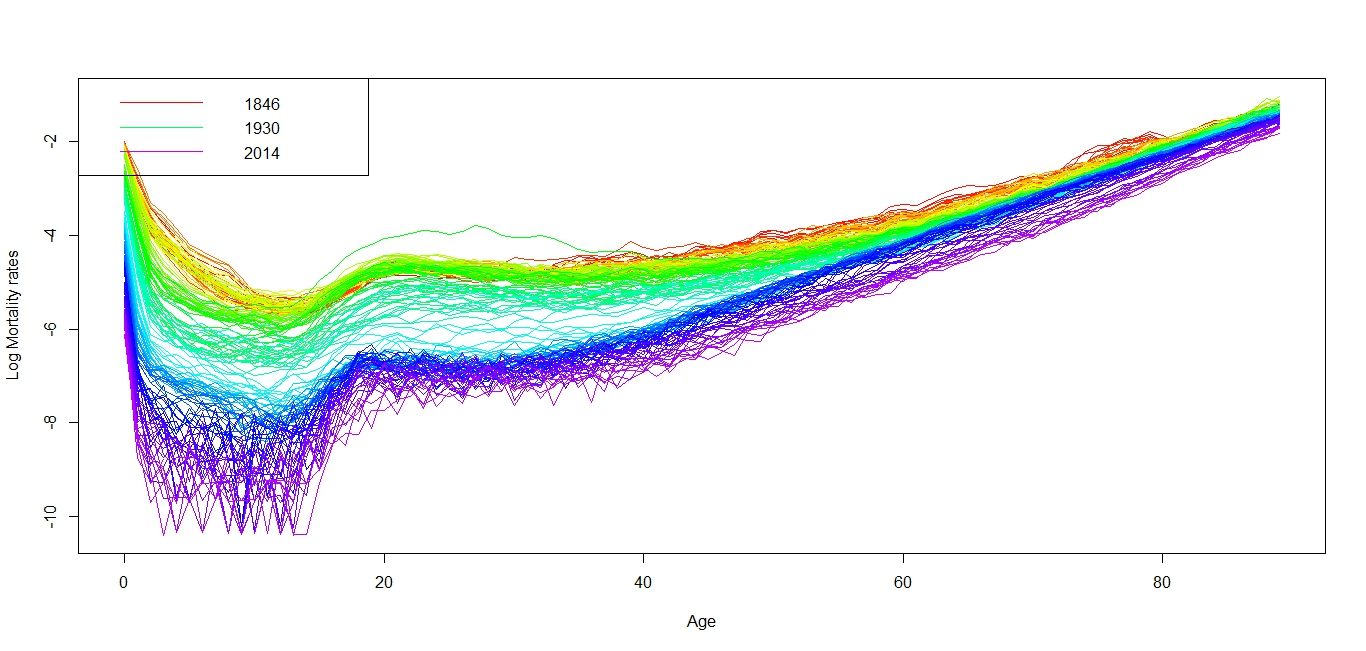
\includegraphics[scale=0.3]{force_mortality_male.jpeg}
  \caption{\textbf{Force of Mortality sexe-neutral}}
  \end{figure}

\end{frame}

%%%%%%%%%%%%%%%%%%%%%%%%%%%%%%%%%%%%%%%%%%%%%%%%%%%%%%

\begin{frame}

\begin{figure}
  \centering
   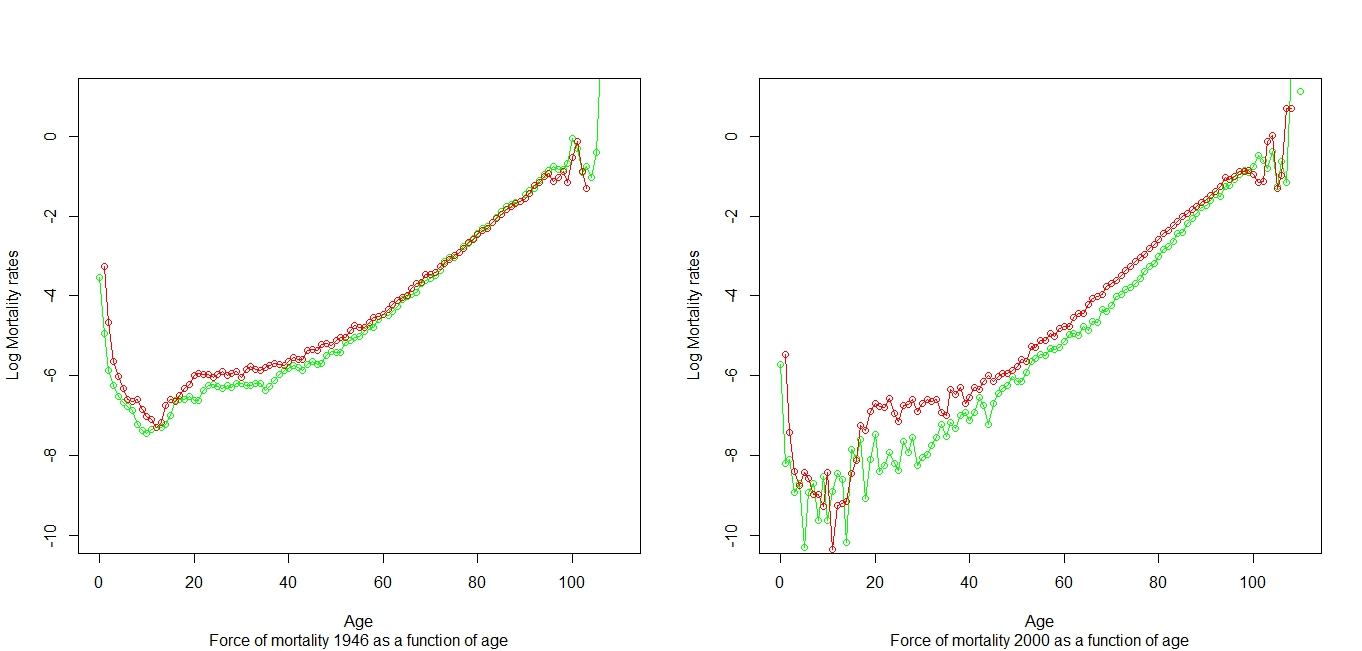
\includegraphics[scale=0.2]{force_mrotality_1946_2000.jpeg}
  \caption{\textbf{Force of Mortality for the years 1946 and 2000}}
  
\end{figure}

\end{frame}
%%%%%%%%%%%%%%%%%%%%%%%%%%%%%%%%%%%%%%%%%%%%%%%%%%%%%%%

\begin{frame}
\frametitle{Mathematical formulation of the model.}

\begin{itemize}
  \item $ l_0$ is the age at the beginning of the contract so $l_0+k$ will be the age at time k; $l_r$ is the age when retirement start.
  \item s is the pension benefit until the maximum realistic age $l_e$.
  \item One-step survival probabilities $_{1}P_l = P_l$ and mortalities $_{1}q_l = q_l = 1- P_l$ . 
  \
  \item  $_{k} P_{l_0}$ is the probability that and individual of age $l_0$ is alive at age $l+k$
  \item d = $1\over{1+r}$ is the discount.
  
\end{itemize}
\end{frame}
%%%%%%%%%%%%%%%%%%%%%%%%%%%%%%%%%%%%%%%%%%%%%%%%%%%%%%%%%%%%%%%%%%%%%%%%%

\begin{frame}

\begin{itemize}
 \item The most popular mathematical description of mortality is the Gomperz-Makeham: \\
  \end{itemize}
  
\begin{block}{Gomperz-Makeham}
 
$ \mu (\textit{l}) = \theta_0 + \theta_1e^{\theta_2l} $ is the intensity.\\
$_kp_l = exp (-\int_{lT}^{(k+l)T}\mu (\textit{l})d_l) $\\
~~~~~$= exp(-\int_{lT}^{(k+l)T}\theta_0 + \theta_1e^{\theta_2l})d_l ) $\\
~~~~~$ = exp(- \theta_0 kT - {\theta_1 \over\theta_2}(e^{\theta_2kT}-1)e^{\theta_2lT})$ \\

The current mortalities  $q_{l0}$ can then be written as: 

$ q_{l0} =  1 - P_{l0} =1 - e ^{-\theta_0 - \theta_1e^{\theta_2l}}$
 
 Where $\theta_0, \theta_1, \theta_2$ are parameters.
 
 \end{block}
\end{frame}
%%%%%%%%%%%%%%%%%%%%%%%%%%%%%%%%%%%%%%%%%%%%%%%%%%%%%%%%%%%
\begin{frame}
\begin{figure}
  \centering
   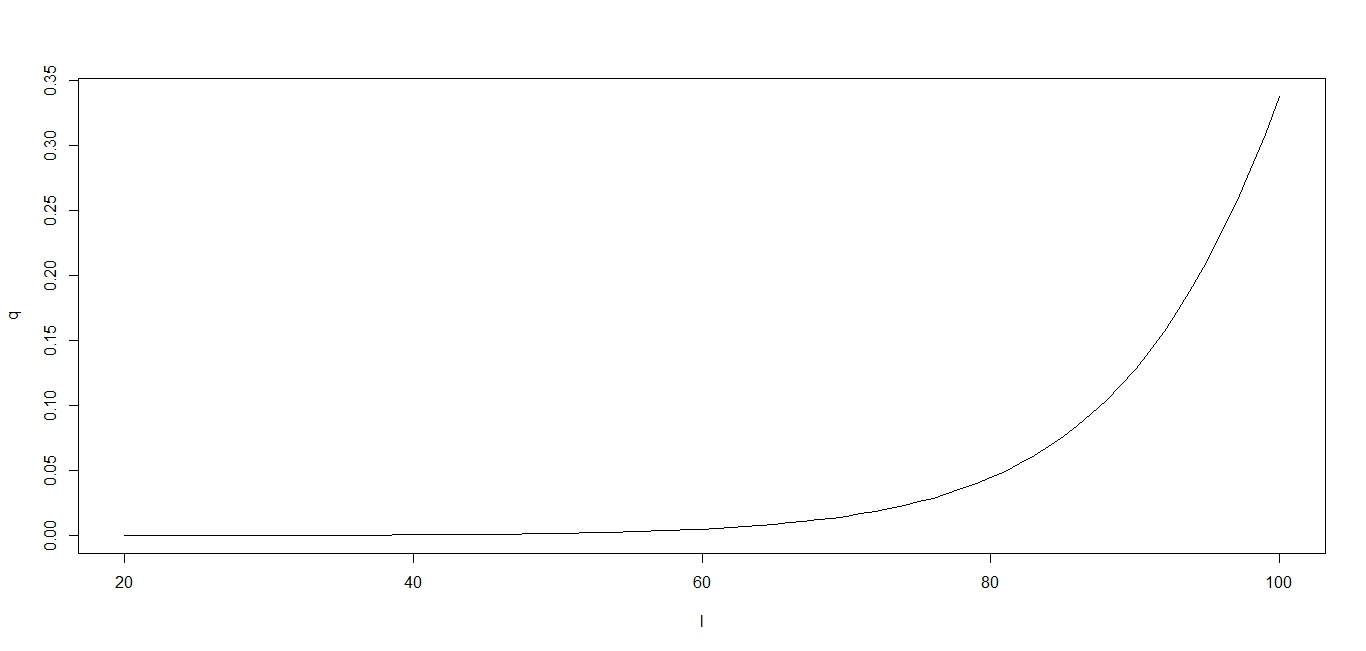
\includegraphics[scale=0.2]{mort_proba_Gromp_Make.jpeg}
  \caption{\textbf{Plot of the true mortalities probabilities under the Gomperz-Mekam.}}
  
  \end{figure}

\end{frame}

%%%%%%%%%%%%%%%%%%%%%%%%%%%%%%%%%%%%%%%%%%%%%%%%%%%%%%%%%%%%%%%%%%%%%%%%%%
\begin{frame}[fragile]


\begin{itemize}
\item The parameters of the Gomperz-Makeham model are difficult to interpret and tell us little about how long we expect people to live.
\item Lee- Carter, we supposed for the model that the life expectancy is
growing. We take the mortality  of an individual of age \textit{l} in year \textit{k}.
\end{itemize}
%\end{frame}



%\begin{frame}[fragile] % Need to use the fragile option when verbatim is used in the slide
%\frametitle{Verbatim}
\begin{block}{Simplified version of the Lee-Carter with parameter estimates for Norway.}

\vspace{5mm}
\hspace{20mm}\scalebox{1.5} {$ q_{lk} = w_l^kq_{lo} $}

Where

\hspace{20mm} \scalebox{1.5}{$\log(w_l) = -b_{0} \frac{e^{h_l}}{(1+e^{h_l})^2} $} ~~~~~~ and~~~~~~~~~~~~\scalebox{1.5}{$ h_l = a_0+a_1l+ a_2l^2 $}



\end{block}

\end{frame}

%%%%%%%%%%%%%%%%%%%%%%%%%%%%%%%%%%%%%%%%%%%%%%%%%%%%%%%%%%%%%%%%%%%%%%%%%%%%%%
\begin{frame}
\frametitle{Dealing with longer lives}
\begin{itemize}


 \item How Mortalities are enter in actuarial calculation.
 
\vspace{5mm}\scalebox{1.6}{ $ {p_l} \,\to\, \textbf{Z}\,\to\,\hat{p}_l\,\to\,_k\hat{p}_l \,\to\, \hat{\pi},\hat{\chi}_k,\widehat{PV_0}   $  }

\vspace{5mm} \item Now people live longer than expected.This can be analyse by introducing a default sequence $q_{l0}$ of mortality. Two approaches can be use her, the cohort version and the time-dynamic version.

\begin{block}{Simple model}

\hspace{5mm}\scalebox{1.6}{$ q_l(i) = q_{l0}e^{-\gamma(i)}$ }, cohort version\\
\hspace{5mm}\scalebox{1.6}{$q_{lk} = q_{l0}e^{-\gamma_{k}}$} , time dynamic-version

\end{block}
\item $\gamma(i)$ and ${\gamma}_k$ are parameters that make the mortalities deviate from the default sequence $q_{l0}$.
\end{itemize}

\end{frame}

%%%%%%%%%%%%%%%%%%%%%%%%%%%%%%%%%%%%%%%%%%%%%%%%%%%%%%%%%%%%%%%%%%%%%%%%%%%%%%%%
\begin{frame}

\begin{block} {k-step survival probabilities required for actuarial calculations.}

\hspace{5mm}\scalebox{1.6}{$ _{k+1}p_l = {1 - q_{l+k}(l)}._kp_l $}, Cohort version.\\
\hspace{5mm}\scalebox{1.6}{$ _{k+1}p_l = (1 - q_{l+k,k})._kp_l $}, time-dynamic version.

\end{block}

\begin{itemize}

\item For k = 0,1,2,..., and people of age l born at -l, the probability that they survive the periode from k to k+1 is then $ 1 - q_{l+k}(l)$ and $ (1 - q_{l+k,k}) $ \\

\item By inserting the simple model into the k-step survival probabilities we obtain:\\

\begin{block} {Life table.}

\hspace{5mm}\scalebox{1.6}{$ _{k+1}p_l = ({1 - q_{l0}^{{-\gamma }(l)}})._kp_l $}, Cohort version.\\
\hspace{5mm}\scalebox{1.6}{$ _{k+1}p_l = ({1 - q_{l0}^{{-\gamma }_k}})._kp_l $}, time-dynamic version.

\end{block}

\end{itemize} 

\end{frame}

%%%%%%%%%%%%%%%%%%%%%%%%%%%%%%%%%%%%%%%%%%%%%%%%%%%%%%%%%%%%%%%%%%%%%%%%%%%%%%%%
\begin{frame}

\begin{itemize}
\item With the appropriate life table $_kp_l $ it is now possible to compute the estimated equivalence premium,liability and present value for k = 1,2,3,...

\item The equivalence premium $\pi$ is the solution of : 

\end{itemize}

 \hspace{20mm} \scalebox{1.5}{$ \pi \sum\limits_{k=0}^{\ l_r-l_0-1} d^{k}\ _{k} p_{l_0}  = s\sum\limits_{k=l_r-l_0}^{\ l_e-l_0} d^{k}\ _{k} p_{l_0} $}

\end{frame}
%%%%%%%%%%%%%%%%%%%%%%%%%%%%%%%%%%%%%%%%%%%%%%%%%%%%%%%%%%%%%%%%%%%


\begin{frame}
\frametitle{Numerically illustrations}
\begin{figure}
  \centering
   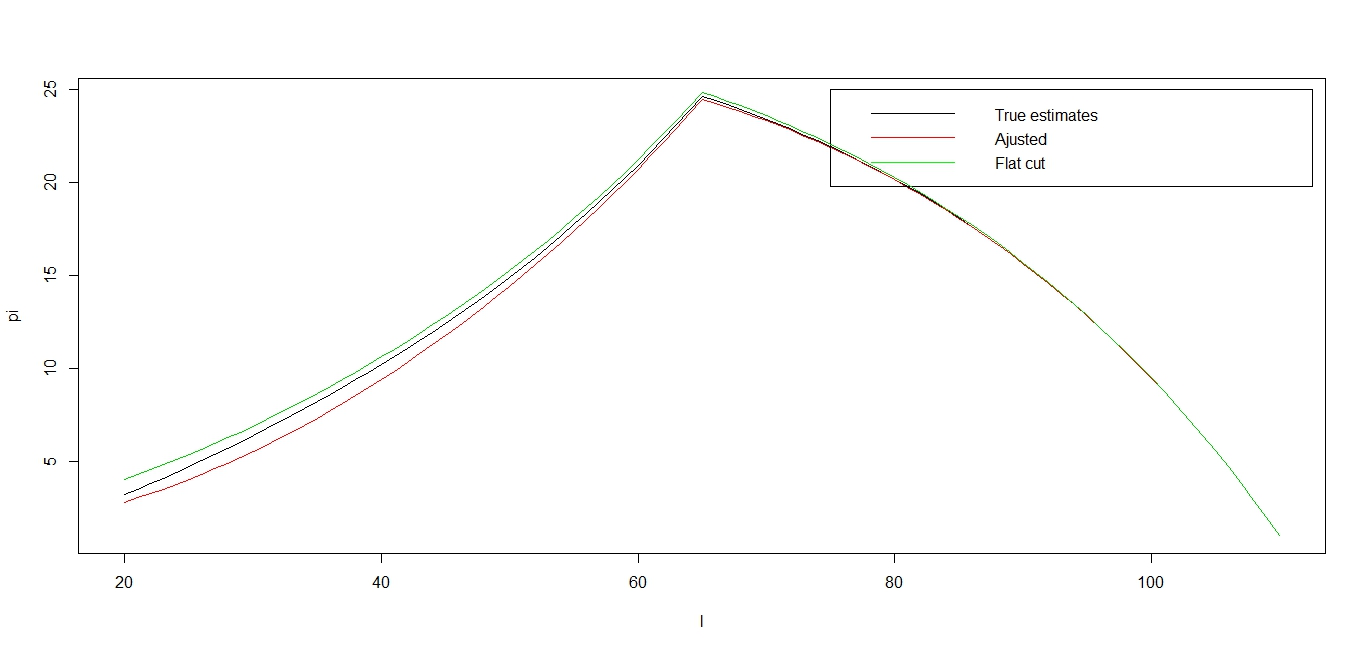
\includegraphics[scale=0.2]{sex_neutral_premia.jpeg}
  \caption{\textbf{One time premia Sex-neutral}}
  
\end{figure}

\end{frame}

%%%%%%%%%%%%%%%%%%%%%%%%%%%%%%%%%%%%%%%%%%%%%%%%%%%%%%%%%%%%%%%%%%%
\begin{frame}

\begin{figure}
  \centering
   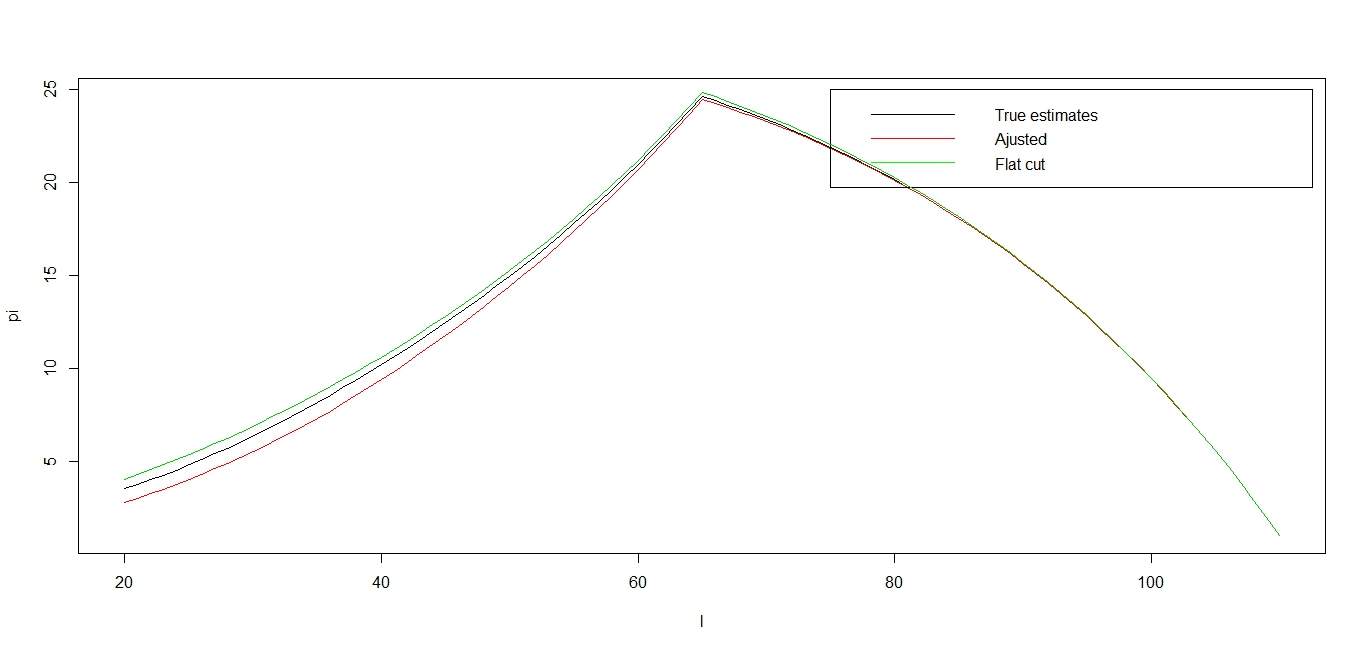
\includegraphics[scale=0.16]{male_premia.jpeg}
  %\caption{\textbf{One time premia male}}
  
\end{figure}
\begin{figure}
  \centering
   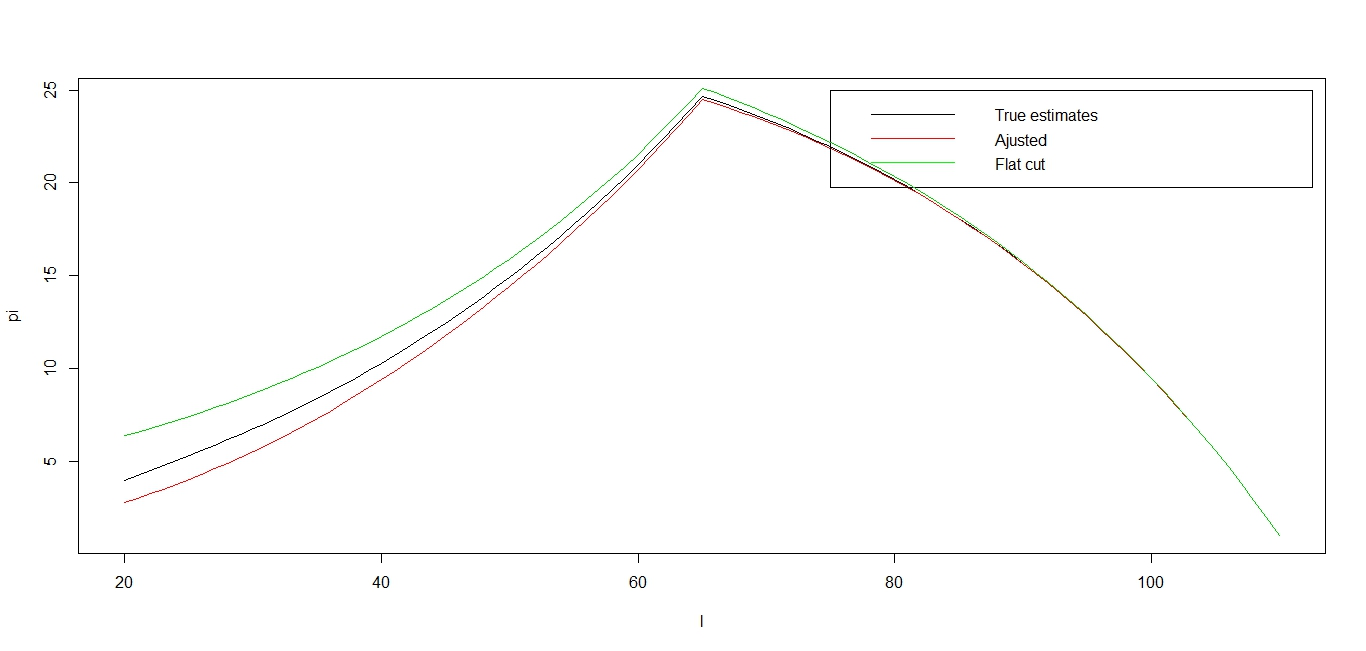
\includegraphics[scale=0.16]{female_premia.jpeg}
  \caption{\textbf{One time premia male and  female}}
  
\end{figure}


\end{frame}



%%%%%%%%%%%%%%%%%%%%%%%%%%%%%%%%%%%%%%%%%%%%%%%%%%%%%%%%%%%%%%%%%%%
\begin{figure}
  \centering
   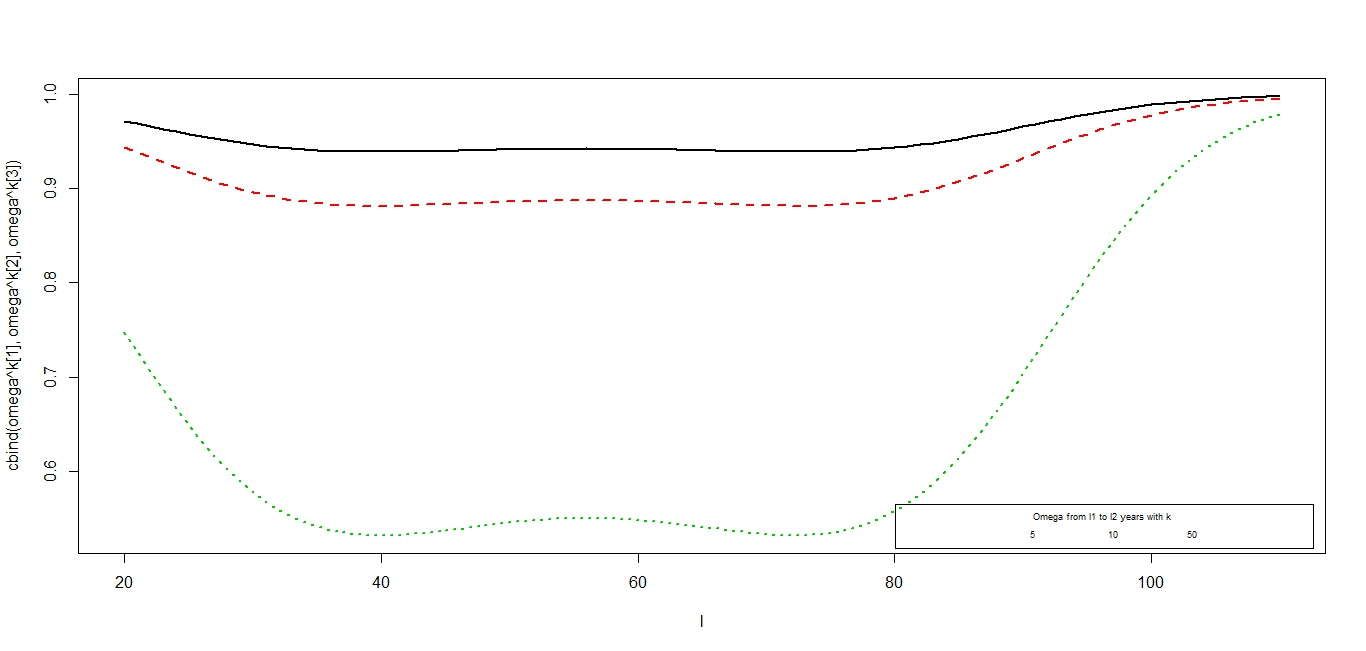
\includegraphics[scale=0.26]{reduction_factor.jpeg}
 % \caption{\textbf{Lee - Carter reduction factor.}}
  
\end{figure}

%%%%%%%%%%%%%%%%%%%%%%%%%%%%%%%%%%%%%%%%%%%%%%%%%%%%%%%%%%%%%%%%%%
\begin{frame}


\begin{itemize}
 \item The lee-carter becaome less smooth over time. The forecast become narrow for people beyon 70.
 \item The model underpredict futurs gains. 
\end{itemize}

\end{frame}
%%%%%%%%%%%%%%%%%%%%%%%%%%%%%%%%%%%%%%%%%%%%%%%%%%%%%%%%%%%%%%%%%%



\begin{frame}

\hspace{30mm} {\textbf{Thank You For your attention !}}

\end{frame}










\end{document} 